\chapter*{Introduction}
\addcontentsline{toc}{chapter}{1. Introduction} % Manual index entry
% Hablar de la empresa
% Hablar del objetivo del trabajo
% Comentar la estructura del documento

PRUEBA GLOSARIO: \gls{tempo}$^{(*)}$


En el mundo actual, donde la eficiencia y la toma de decisiones estratégicas marcan la diferencia entre avanzar o quedarse atrás, la gestión de tareas dentro de una empresa adquiere un papel fundamental.
Muchas veces, detrás de un buen producto o servicio, hay una planificación precisa, una coordinación cuidada y un aprovechamiento óptimo de los recursos disponibles.
En este contexto, las matemáticas, y más concretamente la optimización, se convierten en una herramienta poderosa para transformar la complejidad en soluciones claras y aplicables.

Este trabajo surge con la intención de tender un puente entre el conocimiento teórico y su aplicación práctica en el entorno empresarial.
Hemos elegido como caso de estudio la empresa Intercrop, ubicada en Cartagena, especializada en el sector agroalimentario.
Intercrop destaca por su compromiso con la sostenibilidad y la innovación en la producción agrícola, pero como toda empresa, se enfrenta a retos logísticos y organizativos que requieren soluciones inteligentes.
Intercrop no solo opera a nivel nacional, sino que también mantiene una estrecha relación con el mercado internacional. 
Exporta una parte importante de su producción a distintos países europeos, lo que exige altos estándares de calidad, cumplimiento riguroso de plazos y una logística bien estructurada.
Esta dimensión internacional añade complejidad a su gestión operativa, ya que debe coordinar las tareas agrícolas con los calendarios de transporte, las exigencias fitosanitarias y los compromisos comerciales en el extranjero.
Todo ello convierte a esta empresa en un entorno especialmente interesante para aplicar herramientas de optimización que ayuden a mejorar la planificación y la eficiencia en un contexto real y exigente.

A través de este proyecto, abordaremos el problema de planificación de tareas dentro de la empresa. La meta es diseñar un modelo de optimización que permita organizar de forma eficiente las actividades,
 considerando las restricciones del entorno real: tiempos, recursos limitados, dependencias entre tareas y otros factores logísticos.
Este proceso nos permitirá no solo aportar una propuesta de mejora a la empresa, sino también aplicar de forma práctica los conceptos matemáticos aprendidos en el aula, especialmente en lo que respecta a programación lineal y optimización.
\vspace{10mm}
\begin{figure}[ht!]
    \centering
    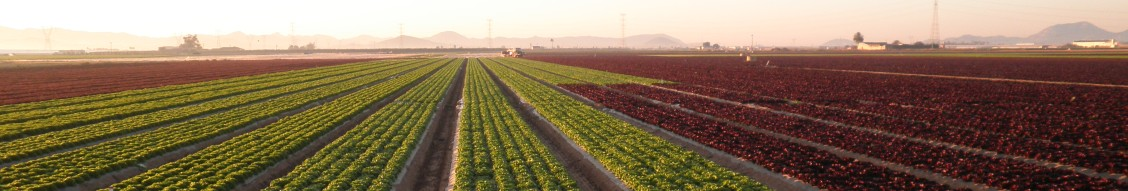
\includegraphics[width=1\textwidth]{img/campitos_lindos.jpeg}
    %\caption{Intercrop, empresa de referencia para el estudio de planificación de tareas agrícolas.}
    \label{fig:campitos_lindos}
\end{figure}

\chapter*{Problem Statement}
\addcontentsline{toc}{chapter}{2. Problem Statement} % Manual index entry
% Explicación en "leguaje natural" del problema
% Simplificaciones
% Descripción de las tareas

La planificación de tareas en el entorno agrícola representa un desafío logístico y operativo considerable,
especialmente en empresas que operan bajo un modelo de producción bajo pedido, como es el caso de Intercrop.
Esta empresa, situada en Cartagena y especializada en productos hortícolas, organiza su producción en función de la demanda estacional.
Durante la campaña de verano, se establecen con antelación tanto la cantidad de kilogramos de producto que se deben suministrar como las fechas específicas de entrega.
Esto implica que toda la planificación de cultivo, desarrollo, cosecha y distribución debe estar ajustada con precisión para cumplir los plazos,
garantizar la calidad del producto fresco (con una vida útil de entre siete y diez días) y minimizar los costes operativos.

El objetivo de este trabajo es abordar, desde un enfoque matemático y práctico, el problema de planificación de tareas agrícolas en el entorno real de esta empresa.
Para ello, nos centraremos en dos cultivos principales: lechuga y espinaca, cada uno con dos variantes específicas.
\begin{itemize}
    \item \textbf{Lechuga}: se cultiva en dos variedades, una de hoja rizada (Apollo, Fig. \ref{fig:apollo}) y otra de hoja lisa (Knox Cos, Fig. \ref{fig:knox}). La lechuga de hoja rizada es más delicada y requiere un cuidado especial. Por su parte, la lechuga de hoja lisa es más resistente y se adapta mejor a condiciones menos precisas.
    \item \textbf{Espinaca}: se cultivan cinco variedades, una de hoja pequeña tanto en su version comun (Baby Spinach, Fig. \ref{fig:baby}) como en su version organica, de hoja mediana tanto de color verde (Teen Spinach, Fig. \ref{fig:teen}) como un color mas rojizo, (Red Spinach, Fig. \ref{fig:red}). También tenemos una 
    una de hoja plana que esta pensada para la realizacion de sopas (Soup Spinach, Fig. \ref{fig:soup})
    En cuanto a las diferencia en el tratamiento, no se encuentran ambios sustanciales en el cuidado.
\end{itemize}
La principal diferencia entre las variedades que estamos tomando es el tiempo de cultivo de cada una de ellas.
\begin{figure}[ht!]
    \centering

    \begin{minipage}[b]{0.45\textwidth}
        \centering
        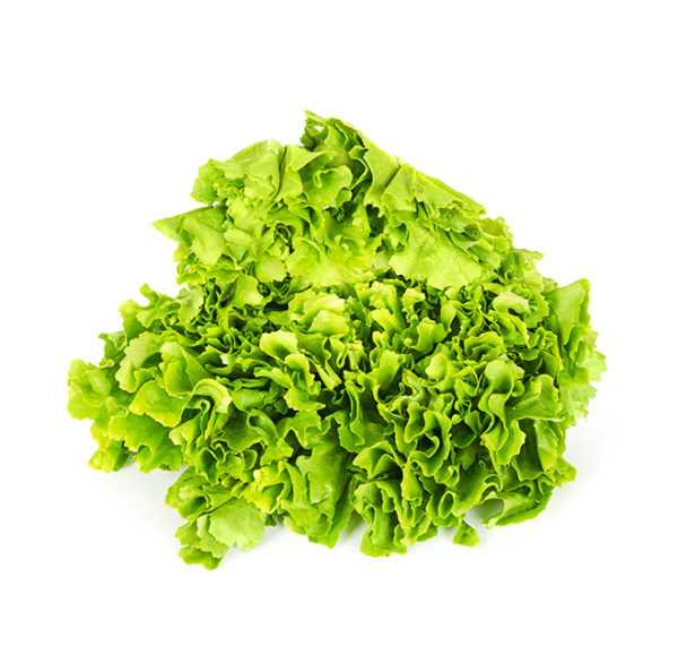
\includegraphics[width=0.7\textwidth]{img/lechuga_apollo.png}
        \caption{Variedad Lechuga Apollo.}
        \label{fig:apollo}
    \end{minipage}
    \hfill
    \begin{minipage}[b]{0.45\textwidth}
        \centering
        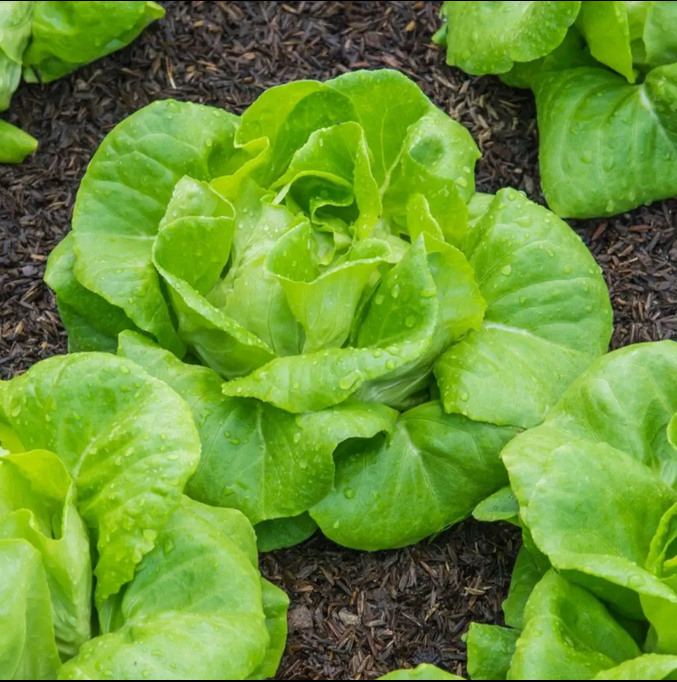
\includegraphics[width=0.6\textwidth]{img/lechuga_knox.png}
        \caption{Variedad Lechuga Knox Cos.}
        \label{fig:knox}
    \end{minipage}

\end{figure}

\begin{figure}[ht!]
    \centering

    \begin{minipage}[b]{0.45\textwidth}
        \centering
        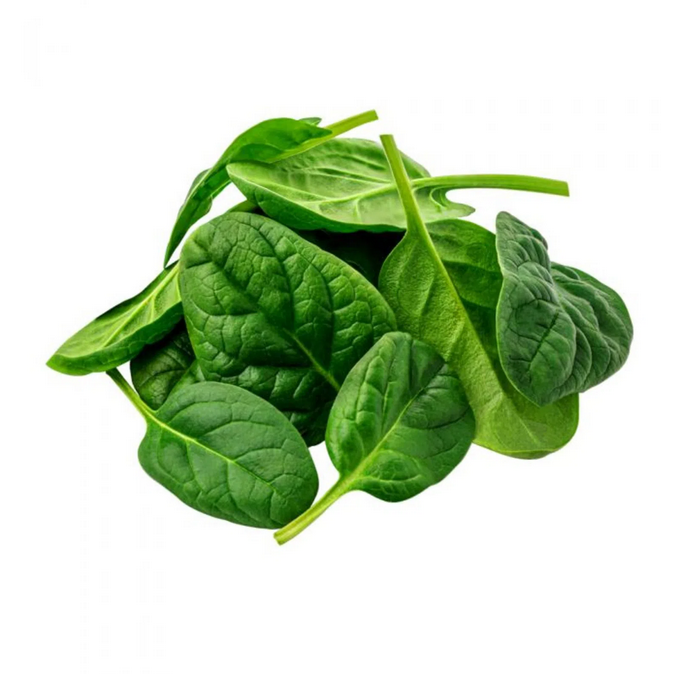
\includegraphics[width=0.7\textwidth]{img/baby_spinach.png}
        \caption{Variedad Baby Spinach.}
        \label{fig:baby}
    \end{minipage}
    \hfill
    \begin{minipage}[b]{0.45\textwidth}
        \centering
        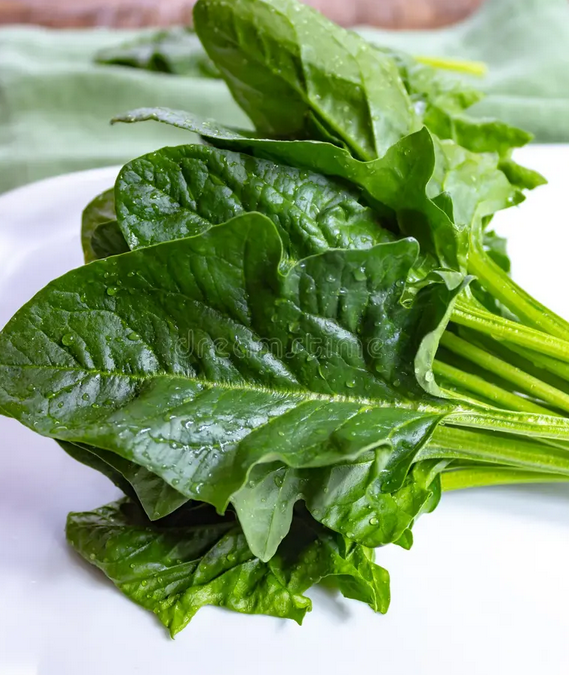
\includegraphics[width=0.6\textwidth]{img/teen_spinach.png}
        \caption{Variedad Teen Spinach.}
        \label{fig:teen}
    \end{minipage}
    \begin{minipage}[b]{0.45\textwidth}
        \centering
        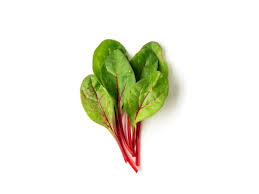
\includegraphics[width=0.6\textwidth]{img/red_spinach.jpg}
        \caption{Variedad Red Chard.}
        \label{fig:red}
    \end{minipage}
    \begin{minipage}[b]{0.45\textwidth}
        \centering
        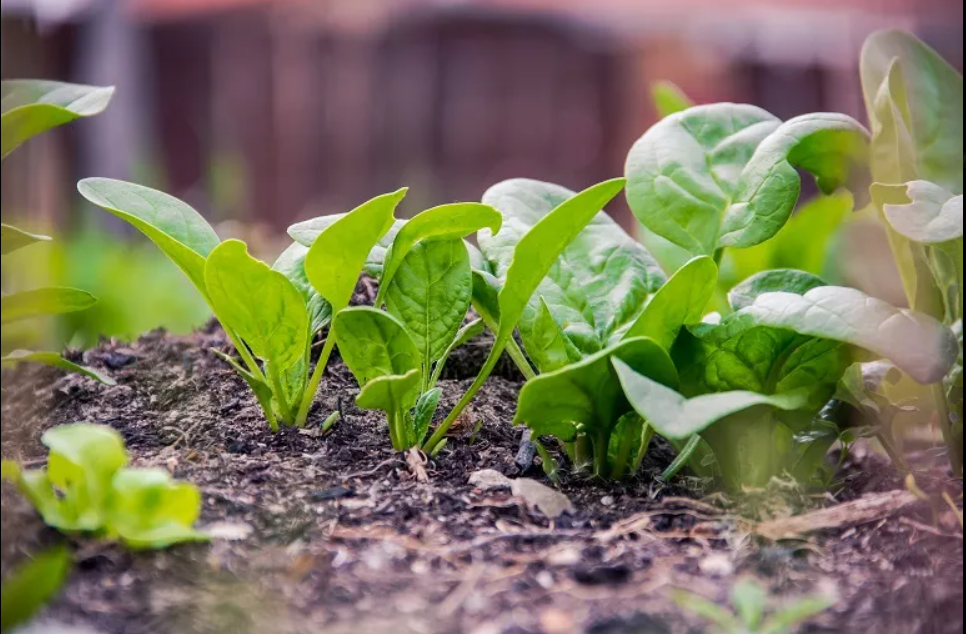
\includegraphics[width=0.6\textwidth]{img/soup_spinach.png}
        \caption{Variedad Soup Spinach.}
        \label{fig:soup}
    \end{minipage}
\end{figure}


Antes de pasar a desglosar las tareas que engloban el proceso de cultivo, es importante destacar una diferencia fundamental entre ambos productos.
La lechuga se trabaja mediante plantación: las semillas se envían a un semillero y posteriormente se trasplantan las plántulas al campo. 
En el caso de la espinaca, se utiliza el método de siembra directa, introduciendo las semillas directamente en la tierra.
Debido al diferente proceder de ambos métodos, cada cultivo tendrá sus tiempos y necesidades específicas, lo que influirá en la planificación de las tareas.

La lista de tareas necesarias para completar un ciclo de cultivo es la siguiente:
\begin{enumerate}
    \item Preparación de la tierra: conjunto de labores inicales donde se rompe y voltea la tierra para airearla, y se abona para dejarla preparada adecuadamente antes del cultivo.
          Seguidamente, mediante maquinaria especializada, se organizan las superficies de cultivo en mesetas.
    \item Colocar papel: se instalan láminas que impiden el crecimiento de malas hierbas, lo que reduce la competencia con el cultivo principal.
    \item Sembrar o plantar: según el tipo de variante, se introducen semillas directamente o se plantan brotes previamente cultivados por una empresa externa.
    \item Riego: instalación de sistemas de riego por aspersión en las laderas de las mesetas, necesarios para el mantenimiento del cultivo.
    \item Colocación de arquillos: se instalan arcos metálicos sobre los cultivos para dar soporte a la protección posterior.
    \item Poner malla: se cubren los arquillos con una malla de poliamida que protege los cultivos y ayuda a mantener la temperatura adecuada para su desarrollo.
    \item Quitar malla: una vez que el cultivo ha madurado, se retira la malla protectora.
    \item Quitar arquillos: tras la retirada de la malla, se procede a desmontar los arquillos metálicos.
    \item Quitar riego: se desmonta el sistema de riego instalado previamente.
    \item Recogida de cosecha: proceso final de recolección, que puede realizarse manualmente (con operarios que colocan los productos en cajas) o de forma automatizada.
\end{enumerate}

Cada una de estas tareas se lleva a cabo con maquinaria distinta, generalmente aperos arrastrados por tractores, lo que implica velocidades de trabajo diferentes según el equipo empleado.
Además, Intercrop organiza su producción mediante grupos de trabajo especializados, que no están contratados desde el inicio de campaña, sino que se van incorporando según se requieren sus funciones.
Esta estructura permite adaptarse a las necesidades del proceso, pero también genera cuellos de botella cuando un grupo debe esperar a que otro finalice su tarea para continuar.

Durante nuestra visita a la empresa, observamos que esta falta de sincronización entre grupos provoca frecuentes horas muertas: periodos en los que los trabajadores están presentes pero sin poder actuar,
ya que el trabajo anterior aún no ha finalizado. Estas horas, aunque no productivas, computan en el total de horas trabajadas y generan un coste económico directo para la empresa.

La presente propuesta tiene como objetivo central la creación de un modelo de planificación que permita minimizar las horas improductivas entre grupos de trabajo,
garantizando al mismo tiempo que se cumplan los plazos de entrega comprometidos. Una coordinación más eficiente de las tareas supondría una mejora significativa en la utilización de los recursos,
reduciendo tiempos de espera y aumentando la productividad general del sistema.

\section*{Simplificaciones del modelo}
\addcontentsline{toc}{section}{2.1. Simplificaciones del modelo} % Manual index entry

Para poder abordar el problema dese un punto de vista matemático y computacional, ha sido necesario realizar algunas simplificaciones, que nos permiten centrarnos en los aspectos esenciales del proceso
sin pérdida de generalidad:
\begin{itemize}
    \item Reducción de escala: el modelo se aplica únicamente a dos fincas, una dedicada a lechuga y otra a espinaca. 
          Esta decisión permite trabajar con dos líneas de producción diferenciadas y representativas, sin necesidad de modelar toda la operación global de la empresa.
    \item Fincas de tamaño medio: se ha asumido que ambas fincas tienen dimensiones similares y medias, lo que permite aplicar el mismo esquema de planificación
          a cada una sin consideraciones de tamaño o forma específicas.
    \item Cultivo homogéneo: se considera que en una misma finca realizaremos las tareas que necesarias para el cuidado de la variedad más delicada. 
          Por tanto, supondremos que en la finca destinada a las lechugas se realizan todas las tareas de la lista mencionada, y en el caso de las espinacas obviaremos el uso de malla y arquillo. 
          Así, en la primera finca se realizarán las 10 tareas mencionadas anteriormente, mientras en la finca correspondiente a las espinacas solo se realizarań las tareas 1, 3, 4, 9 y 10.
    \item Grupos de trabajo independientes: cada cultivo es atendido por  un grupo de trabajo diferente, con su propia maquinaria y recursos.
          Esto permite tratar ambas líneas de producción de manera paralela y simplificada.
    \item Conversión de unidades: las velocidades de la maquinaria, proporcionadas por la empresa originalmente en kilómteros por hora, han sido traducidas a caminos por hora,
          para simplificar la formulación y adaptar las unidades a la estructura del modelo.
    \item Condiciones ideales: el modelo se desarrolla bajo un escenario en el que no hay fallos mecánicos ni interrupciones por causas climáticas.
          Es decir, se asumen que todas las tareas se realizan en el tiempo estimado y que no hay retrasos por factores externos.
    \item Jornada laboral fija: se condidera una jornada laboral de 8 horas diarias, sin cambios estacionales ni festvos.
\end{itemize}
 
Estas simplificaciones no eliminan la complejidad del problema, pero permiten estructurar un modelo realista, funcional y computacionalmente viable que sirva como base para una futura ampliación o implementación práctica.






\chapter*{Formulation}
\addcontentsline{toc}{chapter}{3. Formulation} % Manual index entry
% Variables
% Funcion objetivo
% Restricciones

Para abordar la planificación de tareas agrícolas de manera estructurada y optimizable, hemos construido un modelo matemático que describe formalmente las restricciones, recursos y objetivos del problema planteado.
Esta formulación nos permitirá buscar una asignación eficiente de tareas que minimice los tiempos improductivos, garantizando que las labores se ejecuten de acuerdo a sus requisitos técnicos y temporales.

\section*{Parametros}
\addcontentsline{toc}{section}{3.1. Parámetros} % Manual index entry
Lo primero que necesitamos es definir un conjunto de parámetros que represente correctamente el entorno de trabajo en ambas fincas, cada una dedicada a un producto distinto (lechuga y espinaca),
y por tanto, como se mencionaba anteriormente, con secuencias de tareas diferenciadas.


\subsubsection{Conjunto de tareas}
\begin{itemize}
    \item Conjunto de tareas para la finca 1, destinada a lechuga:
    
    $T_1$:= \{preptierra1,papel1,plantar1,ponerriego1,ponermalla1,quitarmalla1,quitarriego1,cosecha1\}
    \item Conjunto de tareas para la finca 2, destinada a espinaca:
    
    $T_2$:= \{preptierra2,sembrar2,ponerriego2,quitarriego2,cosechar2\}
\end{itemize}

\subsection{Variedades y tiempos de crecimiento}

En cada tierra nos encontramos distintas variedades de un mismo producto, que se encontrarán repartidas de forma homogénea por las mesetas:

\[\begin{aligned}
        Q_1:={apollo, knoxcos}\\
        Q_2:={babyspinach, teenspinach, babyspinachorganic, soupspinach, redspinach}
    \end{aligned}\]

Cada una de ellas tendrá un tiempo de crecimiento:
\[\begin{aligned}
        S_1:=\{s_{apollo},s_{knoxcos}\}\\
        S_2:=\{s_{babyspinach}, s_{teenspinach}, s_{babyspinachorganic}, s_{soupspinach}, s_{redspinach}\}
    \end{aligned}\]



\subsubsection{Mesetas y horizonte temporal}

Para cada tierra, definimos el conjunto de mesetas correspodiente ($M_j$), el número de mesetas totales ($N_j$), y el conjunto de horas ($H$) de trabajo disponibles durante el pedido:
    \[\begin{aligned}
        M_1:=\{1....50\}\\
        M_2:=\{1....90\}\\
        N_1:=50\\
        N_2:=90\\
        H:=\{1...240\}
    \end{aligned}\]

\subsubsection{Disponibilidad temporal de las tareas}

Las tareas no están activas durante todo el horizonte temporal: van entrando escalonadamente. 
Además, como en cada finca habrá distintas tareas disponibles, definimos una familia de horarios para cada una:

\[\begin{aligned}
    H_1 &:= \{H_{preptierra1},H_{papel1},H_{plantar1},H_{ponerriego1},H_{ponermalla1},H_{quitarmalla1},H_{quitarriego1},H_{cosecha1}\}\\
    H_2 &:= \{H_{preptierra2},H_{sembrar2},H_{ponerriego2},H_{quitarriego2},H_{cosechar2}\}   
\end{aligned}\]    

\subsubsection{Velocidad de trabajo de las máquinas}

Cada tarea se realiza con maquinaria diferente, y por tanto a diferentes velocidades. Estas se expresan en mesetas/hora:
\begin{center}
$V_{i_1}:=$ numero maximo de mesetas por camino en una hora $\forall i_1 \in T_1$

$V_{i_2}:=$ numero maximo de mesetas por camino en una hora $\forall i_2 \in T_2$
\end{center}



\subsubsection{Personal asociado a cada tarea}
Cada tarea cuenta con un grupo de trabajo asignado, que incluye un número de personas necesario para su ejecución.
\begin{center}
    $P_{i_1}$ := número de personas asignadas a la tarea $i_1 \in T_1$

    $P_{i_2}$ := número de personas asignadas a la tarea $i_2 \in T_2$    
\end{center}

\section*{Variables de decisión}
\addcontentsline{toc}{section}{3.2. Variables de decisión} % Manual index entry
Para modelar correctamente la ejecución de las tareas en cada meseta y en cada momento del horizonte temporal, se define la siguiente variable binaria:
\[\begin{aligned}
    x_{i_j,k,l} = \begin{cases} 1 & \text{si la tarea } i \text{ se realiza en el camino } k \text{ y en la hora } l \\ 0 & \text{en otro caso} \end{cases}
\end{aligned}\]

donde:
\begin{itemize}
    \item $i_j$ representa una tarea perteneciente al conjunto $T_j$.
    \item $k \in M_j$ representa una de las mesetas en la tierra $j$.
    \item $l \in H_{i_j}$ representa una hora dentro del intervalo de disponibilidad de la tarea $i_j \in T_j$.
\end{itemize}

Por otro lado, para capturar los tiempos de espera u horas muertas entre tareas
(es decir, cuando un grupo de trabajo está disponible pero no puede comenzar porque otra tarea previa no ha terminado en esa meseta), definimos la siguiente variable:
\[\begin{aligned}
    w_{i_j l} = \begin{cases} 1 & \text{si la tarea } i_j \in T_j \text{ se puede asignar todavía a un camino en la hora } l \in H_{i_j} \\ 0 & \text{en otro caso} \end{cases}
\end{aligned}\] 


\section*{Restricciones}
\addcontentsline{toc}{section}{3.3. Restricciones} % Manual index entry
El modelo de planificación agrícola debe garantizar que la ejecución de las tareas se ajusta a las capacidades operativas,
al calendario disponible y al orden lógico del proceso productivo. Para ello, se han definido las siguientes restricciones:
\begin{itemize}
    \item  No podemos asignar más mesetas por hora de los que permite la tarea.
           La velocidad de realización de la tarea la marca el tractor, no podemos asignar más mesetas de los que es posible abarcar en una hora.
           Para ello fijamos una hora y una tarea y recorremos las mesetas. El número que obtenemos no debe ser mayor que el máximo número de mesetas que puede hacer la maquinaria. 
	    \[
            \sum_{k\in M_j}x_{i_j kl} \leq V_{i_j} \hspace{0.5cm} \forall i_j \in T_j, \hspace{0.2cm} l\in H_{i_j}
        \]
    \item  Solo podemos realizar las tareas una única vez en las mesetas donde se puedan realizar.
           Para ello fijamos una meseta y una tarea, obteniendo que la suma en todas las horas de su horario debe ser 1,
           pues de lo contrario la tarea o no se habría realizado (si es 0) o se habría realizado más de una vez. 
        \[
	        \sum_{l\in H_{i_j}}x_{i_j kl} =1 \hspace{0.5cm} \forall i_j \in T_j , k \in M_j
        \]
    \item Las tareas siguen un orden que debemos respetar.
          No podemos realizar la siguiente tarea en una meseta sin haber hecho la anterior.
          Debemos comprobar que en esa meseta se ha hecho la tarea anterior a la que nos toca hacer. 
	
	      Fijamos una meseta, una tarea y una hora, y comprobamos que en las horas previas se ha realizado la tarea anterior. 
        \[
	        x_{i_j kl} \leq \sum_{l' \in H_{prev(i_j)}, l'<l}x_{prev(i_j)kl'} \hspace{0.5cm} \forall i_j\in T_j/\{first(T_j)\}, k\in M_j, l \in H_{i_j}
        \]
	
    \item  Hay que respetar el crecimiento de cada variedad. Una vez puesto el riego la planta comienza a crecer,
           y debe estar un tiempo hasta que crezca. El tiempo depende de la variedad.
           Una vez pasado dicho tiempo, se pueden realizar las tareas posteriores.
        \[
	        x_{\text{quitarmalla}1 kl} \leq \sum_{l'\in H_{\text{ponerriego}1}, l'<l-s_{apollo}}x_{\text{ponerriego}1kl'} \hspace{0.5cm} k\in \{1, ..., 36\}, l\in H_{\text{quitarmalla}1}
        \]
	    Esta misma restricción se da para $s_{knoxcos}$ y en este caso tendríamos que $k \in \{37, ..., 50\}$. 
	
        Para las variedades de la segunda tierra tendremos:
        \[
	        x_{\text{quitarriego}2 kl} \leq \sum_{l'\in H_{\text{ponerriego}2}, l'<l-s_{babyspinach}}x_{\text{ponerriego}2kl'} \hspace{0.5cm} k\in \{1, ..., 45\}, l\in H_{\text{quitarriego}2}
        \]

        Esta misma restricción se da para $s_{teenspinach}, s_{babyspinachorganic}, s_{soupspinach}, s_{redspinach}$ y en este caso tendríamos que $k \in \{46, ..., 50\},\{51, ..., 63\},\{64, ..., 74\},\{75, ..., 90\}$
        respectivamente.

    \item  Por último, necesitamos una restricción que active $w_{i_j l}$, es decir, que nos diga si todavía se puede realizar una tarea en una meseta. 
        \[
	        \displaystyle w_{i_j l}\geq \frac{N_j-\sum_{l'<l, l'\in H_{i_j}, k\in M_j}x_{i_j kl'}}{N_j}
        \]
	
	    En el sumatorio se cuentan las mesetas en las que se ha realizado una determinada tarea. Este cociente será $0$ cuando una tarea se haya realizado en todas las mesetas, y será mayor que 0 y menor que 1, cuando todavía quede alguna meseta por hacer. 
	
\end{itemize}


\section*{Función objetivo}
\addcontentsline{toc}{section}{3.4. Función objetivo} % Manual index entry
Nuestro problema consiste en minimizar las horas muertas de los trabajadores. Y nuestra función objetivo será: 
	\[
	    min\hspace{0.1cm} \sum_{i_j \in T_j, l\in H_{i_j}}P_{i_j}\left(\frac{V_{i_j}-\sum_{k\in M_j}x_{i_j kl}}{V_{i_j}}\right)w_{i_j l}
    \]

    La presencia del producto de variables binarias $x_{i_j kl}$ y  $w_{i_j l}$ hace que la función objetivo inicial sea no lineal.
    Debido a que la optimización lineal es considerablemente más eficiente y permite utilizar algoritmos de resolución estándar más robustos,
    se decidió realizar una linealización del modelo.

    Para ello, introduciremos variables auxiliares definidas como:
    \[
        \delta_{i_j k l}=x_{i_j k l}w_{i_j l} \hspace{0.2cm} \forall i_j \in T_j, k \in M_j, l \in H_{i_j}
    \]
    Estas variables auxiliares se restringen mediante las siguientes condiciones que nos aseguran que su valor es idéntico al del producto:
    \[\begin{aligned}
        \delta_{i_j k l} &\leq x_{i_j k l} \hspace{0.5cm} \forall i_j \in T_j, k \in M_j \hspace{0.2cm} l\in H_{i_j}\\
        \delta_{i_j k l} &\leq w_{i_j l} \hspace{0.5cm} \forall i_j \in T_j, k \in M_j \hspace{0.2cm} l\in H_{i_j}\\
	    \delta_{i_j k l} &\geq x_{i_j k l} + w_{i_j l} -1 \hspace{0.5cm} \forall i_j \in T_j, k \in M_j \hspace{0.2cm} l\in H_{i_j}
    \end{aligned}\]

    Una vez introducidas estas variables auxiliares, la función objetivo queda linealizada como:
	\[
        min\hspace{0.1cm} \sum_{i_j \in T_j, l\in H_{i_j}}P_{i_j}\left(\frac{V_{i_j}w_{i_j l}-\sum_{k\in M_j}\delta_{i_j k l}}{V_{i_j}}\right)
    \]
	Esta nueva formulación mantiene exactamente el mismo sentido original de minimización del tiempo improductivo,
    permitiendo al mismo tiempo aprovechar las ventajas de eficiencia computacional y robustez propias de la optimización lineal.



\chapter*{Data}
\addcontentsline{toc}{chapter}{4. Data} % Manual index entry
% Explicación de los datos
% Tablas

Durante nuestra visita a la empresa, recopilamos todos los datos necesarios para nuestro análisis. 
Posteriormente, la empresa nos facilitó la información que habíamos solicitado.

Para nuestro estudio, asumimos que las fincas tienen una forma rectangular. Hemos tomado finca en la que plantaremos las lechugas de
de 100 x 300 metros, mientras que la finca en la tenemos las espincas es de 180x300 metros. Cada meseta de cultivo mide 1.6 metros de ancho, 
con surcos laterales de 0.4 metros para permitir el paso de la maquinaria. Esto implica que cada camino tendrá unas dimensiones de 2 x 300 metros.
En consecuencia, la primera finca encontraremos 50 caminos con sus respectivas 50 mesetas de cultivo, mientras que en la segunda tendremos 
90 caminos con sus 90 mesetas

Las tareas se encuentran mecanizadas, pues es un tractor con un apero diferente los protegonistas en cada una de ellas. Por lo que tenemos 
que saber la velocidad que puede alcanzar el tractor dependiendo del apero que estemos usando en cada una de las tareas. 
 Aunque la empresa nos proporcionó estos datos en kilómetros por hora (km/h), para facilitar nuestra formulación lo hemos pasado a mesetas por hora.

 \begin{table}[ht!]
    \centering
    \begin{minipage}{0.48\textwidth}
        \centering
        \begin{tabular}{|c|c|c|}
            \hline
            \rowcolor{gray!30} \textbf{\textcolor{grey3}{TASK}} & \textbf{\textcolor{grey3}{SPEED}} &  \textbf{\textcolor{grey3}{WORKERS}}\\ 
            \hline
            Soil preparation   & 2 & 4 \\ \hline
            Install paper      & 4 & 2\\ \hline
            Plant              & 3 & 6\\ \hline
            Sow                & 4 & 5\\ \hline
            Install irrigation & 3 & 2 \\ \hline
            Install hoops      & 3 & 3 \\ \hline
            Install mesh       & 3 & 2 \\ \hline
            Remove irrigation  & 3 & 2 \\ \hline
            Remove mesh        & 4 & 2 \\ \hline
            Remove hoops       & 3 & 2 \\ \hline
            Harvest seeds      & 3 & 7 \\ \hline
            Harvest plants     & 2 & 14 \\ 
            \hline
        \end{tabular}
        \caption{Tabla de tareas, velocidades y trabajadores}
        \label{tab:tareas}
    \end{minipage}
    \hfill
\end{table}
Nuestra planificación está diseñada para organizar un mes de trabajo. Considerando una jornada laboral de 8 horas diarias, 
trabajamos con un total de 240 horas al mes.

Por otro lado, los trabajadores se incorporan a la campaña de manera escalonada. Cada uno de ellos está especializado en una 
tarea específica, lo que da lugar a la formación de grupos de trabajo especializados. El número de trabajadores por grupo varía 
en función de la tarea asignada.

Otro aspecto importante a considerar es el tiempo que tardará en crecer cada variedad. La empresa nos proporcionó esta 
información en días, aunque nos advirtieron que, en el caso de las variedades de espinaca, el tiempo de crecimiento no es fijo,
 ya que depende en gran medida de la radiación solar que reciban. Por esta razón, nos proporcionaron un rango de días en los que 
 suelen ser cosechadas, indicando cuáles variedades tienen una mayor o menor variabilidad en su crecimiento. Con estos datos, 
 realizamos una estimación del momento óptimo para la recolección. Además, como trabajamos en horas, convertimos la escala temporal:
 cada día indicado por la empresa se expresa en nuestra formulación como un período de ocho horas. De esta forma, ajustamos los tiempos 
 de crecimiento a nuestro esquema de trabajo.
\begin{table}[ht!]
    \centering
    \begin{minipage}{0.48\textwidth}
        \centering
        \begin{tabular}{|c|c|c|}
            \hline
            \rowcolor{gray!30} \textbf{\textcolor{grey3}{RANGES}} & \textbf{\textcolor{grey3}{DAYS}} &  \textbf{\textcolor{grey3}{HOURS}}\\ 
            \hline
            Baby spinach   & 24 & 192 \\ \hline
            Baby spinach organics  & 34.5 & 208\\ \hline
            Red Spinach              & 22 & 176\\ \hline
            Teen Spinach           & 31.2 & 187\\ \hline
            Soup Spinach & 33.8 & 203 \\ \hline
            Knox Cos     & 22 & 176 \\ \hline
            Apollo      & 24 & 192 \\ \hline
             
            \hline
        \end{tabular}
        \caption{Tabla de Variedades y tiempo de crecimiento}
        \label{tab:Variedades}
    \end{minipage}
    \hfill
\end{table}
\chapter*{Code}
\addcontentsline{toc}{chapter}{5. Code} % Manual index entry\addcontentsline{toc}{chapter}{5. Code} % Manual index entry
% Explicación del código
% Código

\chapter*{Results}
\addcontentsline{toc}{chapter}{6. Results} % Manual index entry
Al dividir el código nuestro resultado será la suma de las dos funciones objetivo que nos han salido
% Tablas
% Gráficos

\chapter*{Conclusion}
\addcontentsline{toc}{chapter}{7. Conclusion} % Manual index entry
El presente trabajo ha permitido abordar un problema real de planificación agrícola desde una perspectiva matemática,
aplicando herramientas de optimización para mejorar la organización del trabajo en la empresa Intercrop.
A través del análisis de las distintas tareas necesarias para el cultivo de lechuga y espinaca —dos productos clave en la producción de la empresa—
se ha puesto de manifiesto la complejidad operativa asociada a la coordinación de equipos, maquinaria y tiempos de ejecución.

A lo largo del proyecto se ha desarrollado un modelo simplificado, pero representativo,
que tiene como objetivo principal minimizar las horas improductivas entre los grupos de trabajo.
Este enfoque responde a una problemática observada directamente en campo:
la existencia de tiempos de espera innecesarios cuando una tarea no puede comenzar hasta que otra finaliza.
Estas horas muertas, aunque inevitables en cierta medida, suponen un coste directo para la empresa y reducen la eficiencia global del sistema productivo.

El modelo ha sido construido considerando dos fincas independientes, cada una con su línea de producción,
y una secuencia de tareas que incluye desde la preparación del terreno hasta la recolección.
A pesar de las simplificaciones introducidas —como la homogeneización del tamaño de las fincas,
la ausencia de condiciones climáticas adversas o la separación estricta entre los grupos de trabajo—, el planteamiento conserva una estructura lógica fiel al proceso real,
permitiendo extraer conclusiones prácticas y escalables.

El desarrollo del trabajo ha demostrado cómo los conocimientos matemáticos adquiridos en el aula pueden ser aplicados con éxito a problemas reales,
aportando soluciones concretas y cuantificables a situaciones cotidianas del entorno profesional.
Además, ha abierto una vía interesante para seguir profundizando en el uso de modelos de optimización en contextos agrícolas,
donde las decisiones eficientes pueden traducirse en mejoras significativas de rendimiento y rentabilidad.

En futuras fases, se podrían incorporar elementos adicionales al modelo, como la variabilidad climática,
los imprevistos mecánicos o la disponibilidad parcial de maquinaria y personal.
También sería interesante extender el estudio a varias fincas interconectadas o explorar estrategias de contratación y rotación del personal más flexibles.
Todo ello contribuiría a construir una herramienta aún más robusta para la toma de decisiones en la gestión diaria de empresas como Intercrop.

\newpage
------------------------------

- Topo
- Apero
- Siembra
- Plantación
- Meseta
- Arquillo
- Malla
- Papel
- Farm lanes: caminos entre las mesetas para el paso de la maquinaria.
- Semillero
